\documentclass[12pt,a4paper]{article}
\usepackage{indentfirst}
\usepackage{anysize} % Soporte para el comando \marginsize
%\marginsize{1.5cm}{1.5cm}{0.5cm}{1cm}
\marginsize{2,5cm}{1,8cm}{2.5cm}{1,7cm}
\usepackage[psamsfonts]{amssymb}
\usepackage{amssymb}
\usepackage{amsfonts}
\usepackage{amsmath}
\usepackage{amsthm}
\usepackage{stackrel}
\usepackage{here}
\usepackage{graphicx}
\usepackage{verbatim}


\usepackage[colorinlistoftodos]{todonotes}
%Color a las referencias
\usepackage[colorlinks=true, allcolors=blue]{hyperref}
\usepackage[spanish]{babel}
\selectlanguage{spanish}
\usepackage[utf8]{inputenc} 

\usepackage{multicol}
\renewcommand{\thepage}{}
\columnsep=7mm

%%%%%%%%%%%%%%%%%%%%%%%%%%%%%%%%%%%%%%%%
\newtheorem{mydef}{Definici\'on}[section]
\newtheorem{mynote}{Nota}[section]
\newtheorem{mytheo}{Teorema}[section]
\newtheorem{myexamp}{Ejemplo}[section]
\newtheorem{mycorol}{Corolario}[section]
\newtheorem{prueba}{Prueba}[section]
\newtheorem{prueba*}{Prueba}[section]
\newtheorem{observacion}{Observaci\'on}[section]
\newtheorem{lema}{Lema}[section]
\newtheorem{solucion*}{Soluci\'on}[section]
\newtheorem{algoritmo}{Algoritmo}[section]
\newtheorem{proposicion}{Proposici\'on}[section]

\linespread{1.4} \sloppy

\newcommand{\R}{\mathbb{R}}
\newcommand{\N}{\mathbf{N}}
\newcommand{\C}{\mathbb{C}}
\newcommand{\Lr}{\mathcal{L}}
\newcommand{\fc}{\displaystyle\frac}
\newcommand{\ds}{\displaystyle}

\DeclareMathOperator{\Dom}{Dom}

%%%%%%%%%%%%%%%%%%%%%%%%%%%%%%%%%%%%%%%%

\renewcommand{\thefootnote}{\fnsymbol{footnote}}
\usepackage{url}
\usepackage{hyperref}


\begin{document}
\begin{center}
 {\Large \textbf{TIRO EN DIANA}}
\end{center}
\begin{center}
 Gustavo Lozano$^{1}$, Miller Silva$^{2}$, Guillermo Borjas$^{3}$, Mirian Geronimo$^{4}$, Ayrton Coronado$^{5}$ \vskip5pt
 {\it Facultad de Ciencias$^1$, Universidad Nacional de Ingenier\'{\i}a$^1$\\}\vskip5pt
 Email: glozanoa@uni.pe$^{1}$, miller.silva.m@uni.pe$^{2}$, gborjasc@uni.pe$^{3}$, mgeronimoa@uni.pe$^{4}$, acoronadoh@uni.pe$^{5}$
\end{center}
%\maketitle 
\vspace*{1cm}
\begin{abstract}

\noindent El estudio de las matrices es fundamental para todo aquel que desea sumergirse en el maravilloso mundo de las matemáticas. Las matrices son parte escencial de ésta y son ampliamente usadas en diversas áreas como lo es en el álgebra lineal, el análisis numérico y las probabilidades. Por ejemplo, para modelar el comportamiento de la propagación de un virus ``T'', se usa la potenciación de matrices; supongamos que tenemos una población de personas sanas ($S$) e infectadas ($I$) donde las personas sanas tienen un $80\%$ de probabilidad de no infectarse en 2 días, y que además hay una cura con $1\%$ de efectividad, estos datos se ordenan en una matriz $A$. Luego si empezamos con una población de 99 personas sanas y 1 infectado, dentro de 2 días tedríamos que la nueva población es: 
\begin{equation*}
\begin{pmatrix} S\\I \end{pmatrix}_2 
=
\begin{pmatrix} 0.8 & 0.01\\0.2&0.99 \end{pmatrix} 
\begin{pmatrix} 99\\ 1 \end{pmatrix}_0
=
\begin{pmatrix} 79.21 \\ 20.79 \end{pmatrix}_2, 
\end{equation*}
es decir que aproximadamente tendríamos 79 personas sanas y 21 infectadas; y ¿qué pasaría en $2n$ días?, bueno tendríamos que la población sería $A^nX_0$. Es aquí donde comienzan las complicaciones, dado que elevar una matriz a su n-ésima potencia no es tarea fácil, sin embargo existe una maravillosa herramienta matemática que nos ayudará a simplificar los cálculos; nos referimos a la matriz de Jordan. La matriz de Jordan satisface $A^n=PJ^nP^{-1}$, lo cual aplicando esto a nuestro problema anterior tendríamos que:
\begin{equation*}
A^n=
\begin{pmatrix} 0.8 & 0.01\\0.2&0.99 \end{pmatrix}^n
=
\begin{pmatrix} -0.05&-0.71\\ -1.00 &0.71 \end{pmatrix}
\begin{pmatrix} 1&0\\ 0 &0.79  \end{pmatrix}^n
\begin{pmatrix} -0.05&-0.71\\ -1.00 &0.71 \end{pmatrix}^{-1}
\end{equation*}
ahora si $n$ es muy grande obtenemos:
\begin{equation*}
\begin{pmatrix} 1&0\\ 0 &0.79  \end{pmatrix}^n
\rightarrow
\begin{pmatrix} 1&0\\ 0 &0 \end{pmatrix}
\Rightarrow
A^n\rightarrow \begin{pmatrix} 0.05&0.05\\ 0.95 &0.95 \end{pmatrix}
\end{equation*}
finalmente cuando $n\to\infty$ la población esperada es:
\begin{equation*}
\begin{pmatrix} S\\I \end{pmatrix}_\infty
=
\begin{pmatrix} 0.05&0.05\\ 0.95 &0.95 \end{pmatrix}
\begin{pmatrix} 99\\1 \end{pmatrix}
=\begin{pmatrix} 4.76\\95.24 \end{pmatrix},
\end{equation*}
esto es, 5 personas sanas y 95 infectadas; ¿increíble verdad?.

Vemos así que \textit{la matriz de Jordan} es muy útil para simplificar operaciones; el desafío es hallarla; para esto es necesario calcular los valores propios de $A$, los cuales podemos obtener usando algunos métodos del análisis numérico tales como \textit{el método potencia, potencia inversa y QR}. Para nuestra suerte ya se conoce la forma general de la potencia  $n-$ésima de la matriz de Jordan.

Este trabajo se centra en calcular la potencia $k-$ésima de una matriz $A\in\R^{12\times 12}$ (\textit{la matriz de puntuación}), la cual contiene puntuaciones de una prueba de tiro en dianas realizados por un cadete, para esto calcularemos su matriz de Jordan asociada, ayudándonos de los métodos numéricos ya mencionados y algunos otros algoritmos de apoyo para calcular los valores propios y los bloques de Jordan.
\end{abstract}

\begin{quotation}
	{\small
		\noindent\textbf{Palabras Clave:} \\ 
	La matriz de Jordan, Método potencia , Método potencia inversa, Método QR, Matriz de puntuación \\
	}
\end{quotation}

\renewcommand{\abstractname}{Abstract}
\begin{abstract}
	\noindent The study of matrices is fundamental for anyone who wants to immerse themselves in the wonderful world of mathematics, since matrices are found in areas such as linear algebra and numerical analysis. Operations with matrices can be easy, such as adding or subtracting matrices, or very hard to multiply or find the inverse, all depending on the order of the matrix. Imagine that we would like to find the ten power of a matrix $A\in\mathbb{R}^{12\times 12} $, to want to calculate it directly would be a crazy thing; for these cases, mathematicians recommend working with a diagonal matrix that is similar to $A$ this is $A=PDP^{-1}$ which verifies $A^n=PD^nP^{-1}$ , where to find the $D^n$ it's much easier than $A^n$. With this we could be calm but ¿What happens if the matrix is not similar to any diagonal matrix? We can still keep calm because in this case we can use Jordan's canonical form of the matrix  $A$, with which it is also true that $A^n=PJ^nP^{-1}$. \textit{The matrix of Jordan} is a nice mathematical tool that helps us to simplify operations, for our luck we already know the general form of $n$-th power of the matrix of Jordan, the `` difficult '' now is to know how to find it; to find it, it is necessary to calculate the eigenvalues of $A$, this can be done using numerical analysis tools such as \textit{the power method, inverse power and QR}. This work focuses on calculating the k-th power of a matrix A (\textit{the scoring matrix}), for this we will use the aforementioned lines.
\end{abstract}


\begin{quotation}
	{\small
		\noindent \textbf{Keywords:} \\ 
		The matrix of Jordan, The power method , The inverse power method, The method QR, The scoring matrix \\
	}
\end{quotation}

\newpage

\begin{multicols}{2}
\section{Introducción}

\noindent En la Academia General Militar de Zaragoza se lleva a cabo la preparación física y técnica de los alumnos o cadetes para la superación de sus respectivos planes de estudio. La creación de hábitos deportivos en los cadetes es fundamental. Es decir, les presentan diferentes deportes militares (orientación, patrullas de tiro, pentatlón militar y concurso de patrullas) y se les inicia en equitación y la defensa personal militar.\\
\noindent Ahora centrémonos solo en el deporte de tiro. Dicha práctica de tiro realizada por los cadetes, consiste en acertar a un objetivo utilizando algún proyectil.\\ Se hace llamar blanco de tiro (y de manera más general, blanco) al objeto que se desea alcanzar con el proyectil, cuando se hace fuego dirigiendo hacia él la puntería. Si se le «hiere», se dice que «se ha dado en el blanco» o «que se ha hecho blanco». \\
\noindent El blanco de tiro característico es un cuadrado de cartulina con anillos concéntricos que suelen ser de color rojo, negro y blanco. El objetivo de las prácticas de tiro al blanco es alcanzar con series de disparos el  centro que lleva un disco pintado de color negro, este recibe el nombre de diana y sirve para marcar de un modo bien visible el sitio adonde se debe dirigir la puntería.
\begin{center}
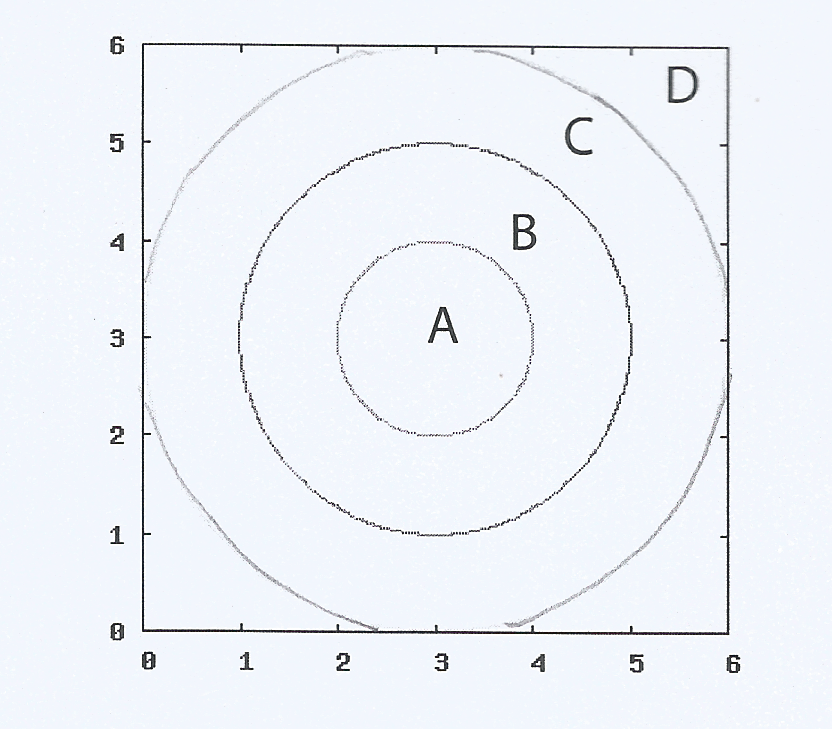
\includegraphics[scale=0.25]{diana.png}\\
Fig1: Diana que se usará en este trabajo.
\end{center}
\noindent En este proyecto analizaremos la práctica de tiro de un cadete en particular. Para este cadete, se dispone de 12 dianas  y en cada diana realizará 12 disparos. Las puntuaciones de cada disparo se ordenan en una matriz $A \in \mathbb{R}^{12\times 12}$ (\textit{matriz de puntuación de la semana 1}). Suponiendo que la \textit{matriz de puntuación de la semana $n$ }esta dada por $A^n$ y la \textit{puntuación final de tiro de la semana $n$ }está dada por la norma de la matriz ($||A^n||_1\text{ o }||A^n||_\infty$), se desea hallar la puntuación final de tiro de la semana 10 usando ambas normas y concluir con qué norma sale más beneficiado el cadete.

\noindent La dificultad de este trabajo se centra en encontrar una expresión general para la potencia $n-$ésima de la matriz $A$, para esto vamos a usar la matriz de Jordan de $A$ ($J_A$) ya que se cumple $A^n=P^{-1}J^n_AP$, donde la potencia  $J^n_A$ es más fácil de hallar comparado a $A$.


\section{Fundamento Teórico}

\noindent Para dar con la descomposición canónica de Jordan de una matriz debemos introducir algunos conocimientos previos:

\begin{mydef}[Operadores Lineales Nilpotentes]
	El operador $T:V\to V$ es nilpotente si $T^{p} = 0$, para algún $p\in\mathbb{N}$. Además se dice que $k\in\mathbb{N}$ es el índice de nilpotencia de $T$ si $$T^{k-1}\neq 0 \ \wedge \ T^{k} = 0$$
\end{mydef}

\begin{mytheo}\label{theo_nilpotentes}  
    \noindent Sea $T:V\to V$, $V$ un $\mathbb{C}$ espacio vectorial, $\dim V = n$, $T$ nilpotente de índice $q$. Luego para $v\in V \ | \ T^{q-1}v\neq 0$, tenemos:
	\begin{enumerate}
		\item El conjunto $\{T^{q-1}v, T^{q-2}v,\ldots,Tv, v\}$ es L.I.
		\item S = $\left<\{T^{q-1}v, T^{q-2}v,\ldots,Tv, v\}\right>$ es invariante por $T$.
		\item Existe un subespacio $U$ de $V$, invariante por $T$ tal que:
		$$V = S\oplus U$$
	\end{enumerate}
\end{mytheo}

\begin{mycorol}
	Del teorema $(\ref{theo_nilpotentes})$
	\begin{align*}
		S &= \left<\{T^{q-1}v, T^{q-2}v,\ldots,Tv, v\}\right>\\
		&\Rightarrow\dim (S) = q\\			
	\end{align*}
%	Luego 
%	\begin{align*}
%		T(S) &= \left<\{T^{q-1}v, T^{q-2}v,\ldots,T^{2}v, Tv\}\right>\\
%		&\Rightarrow\dim T(S) = q-1\\\\
		%T^{2}(S) &= \left<\{T^{q-1}v, T^{q-2}v,\ldots,T^{3}v, T^{2}v\}\right>\\
		%&\Rightarrow\dim T^{2}(S) = q-2
%	\end{align*}
    Inductivamente 
	\begin{align*}
		T^{r}(S) &= \left<\{T^{q-1}v, T^{q-2}v,\ldots,T^{r+1}v, T^{r}v\}\right>\\
		&\Rightarrow\dim T^{r}(S) = q-r\\			
	\end{align*}
\end{mycorol}
\begin{mytheo}
\noindent Sea $T:V\rightarrow V$, dimV=n. Entonces existen $U, W \subset V$ invariantes por T tal que :
\begin{itemize}
    \item $V=U\oplus W$ 
    \item $T|_{U}:U\rightarrow U$ nilpotente  y\\ $T|_{W}:W\rightarrow W$ inversible
\end{itemize}
\end{mytheo}
\noindent\textbf{NOTA:}
\noindent Como $T|_{U}:U\rightarrow U$ es nilpotente entonces existe $q\in\mathbb{N} \ | \  \left(T|_{U}\right)^{q}=0 $ y $(T|_{U})^{q-1}\neq 0$. Ahora hallamos un $v\neq0$ tal que $(T|_{U})^{q-1}v\neq 0$. Así definimos 
$$B_{1}=\{(T|_{U})^{q-1}v, (T|_{U})^{q-2}v, ..., (T|_{U})v,v \},$$ el cual es una base de U . Como W es invariante por T podemos definir $T|_{W}:W\rightarrow W$. Y volviendo a aplicar el teorema anterior $\exists \ U_{2}, W_{2} \subset W$ invariantes por $T$ tal que  $W=U_{2}\oplus W_{2}$,
$T|_{U_{2}}: U_{2}\rightarrow U_{2}$ es nilpotente y $T|_{W_{2}}:W_{2}\rightarrow W_{2}$ inversible.\\
Como $T|_{U_{2}}:U_{2}\rightarrow U_{2}$ es nilpotente, $\exists \ q_{2} \in \mathbb{N}$ tal que $ (T|_{U_{2}})^{q_{2}}=0$ y $(T|_{U_{2}})^{q_{2}-1}\neq 0$, además  $q_{1}=q\geq q_{2}.$
Ahora hallando un $v_{2}\neq0$ tal que $ (T|_{U_{2}})^{q_{2}-1}v_{2}\neq 0$  se puede definir
$$B_{2}=\{(T|_{U_{2}})^{q_{2}-1}v_{2}, (T|_{U_{2}})^{q_{2}-2}v_{2}, ..., (T|_{U_{2}})v_{2},v_{2} \}$$ el cual es una base para $U_{2}$. Luego de manera recursiva obtenemos: \\
$$V=U_{1}\oplus U_{2}\oplus U_{3}\oplus ... \oplus U_{k},$$ donde $U_{1}=U$. Luego $B=\displaystyle\bigcup\limits_{i=1}^{k}B_{i} $ es base de $V$ y además \\
$$\left [T\right]_{B}=\begin{bmatrix}
	\left[T_{|U_{1}}\right]_{\beta_{1}}	&	O	&	\ldots	&	O\\
	O	&	\left[T_{|U_{2}}\right]_{\beta_{2}}	&	\ldots	&	O\\
	\vdots	&	\vdots	& \ddots	& \vdots\\
	O	&	O	&	\ldots	&	\left[T_{|U_{k}}\right]_{\beta_{k}}
\end{bmatrix}$$
 Donde 	$\left[T_{|U_{j}}\right]_{\beta_{j}}=\begin{bmatrix}
		0	&	1	&	0	&	0	&	\ldots	&	0\\
		0	&	0	&	1	&	0	&	\ldots	&	0\\
		0	&	0	&	0	&	1	&	\ldots	&	0\\
		\vdots	&	\vdots	&	\vdots	&	\vdots	&	\ddots	&	\vdots\\
		0	&	0	&	0	&	0	&	\ldots	&	1\\
		0	&	0	&	0	&	0	&	\ldots	&	0\\
	\end{bmatrix}_{q_{j}\times q_{j}}$

\vspace{0.7cm}

\begin{mytheo}[Forma Canónica de Jordan]
	Sea $V$ un $\mathbb{C}$-espacio vectorial, $\dim V = n$, $$T:V\rightarrow V$$ un operador lineal, $\lambda_{1},\lambda_{2},\ldots,\lambda_{k}\in \wedge(T)$ y $n_{1}, n_{2},\ldots , n_{k}$ las multiplicidades algebraicas de los valores propios (respectivamente), entonces:

Existen subespacios $V_{1}, V_{2},\ldots, V_{k}$ invariantes por $T\;\left(T(V_{i})\subseteq V_{i}\right)$ tales que:
\begin{enumerate}
	\item	$V = V_{1}\oplus V_{2}\oplus\ldots\oplus V_{k}$
	\item $\dim V_{i} = n_{i},\quad i=1-k$
	\item El operador $T-\lambda_{i}I:V_{i}\rightarrow V_{i}$ es nilpotente, $i=1-k$. (Aquí se aplica la propiedad ya antes mencionada para un operador nilpotente)
	
	
\end{enumerate}
\end{mytheo}
\noindent Ahora introduciremos algunos métodos numéricos que nos permiten calcular los valores y vectores  propios de una matriz, los cuales son necesarios para construir la forma canónica de Jordan de una matriz.
\subsection{Método potencia}
\noindent Dada una matriz $A\in \mathbb{R}^{n\times n}$, este método calcula el mayor valor propio de $A$ y el vector propio asociado a este valor propio, mediante iteraciones.
Es decir, dada la siguiente relación de recurrencia :\begin{equation*}
    q^{(k+1)} = \frac{1}{\phi_{k}}Aq^{(k)},\quad donde\;\phi_{k} = \Vert Aq^{(k)}\Vert    
\end{equation*} e inicializando con algún vector $q^{(0)}$, al realizar las iteraciones la sucesión converge al autovector asociado al mayor valor propio.


\subsubsection{Convergencia del Método Potencia}
\begin{itemize}
\item Caso general:\\
Sea $\wedge(A)=\{\lambda_{1},\ldots,\lambda_{k}\}$ el esprectro de $A$ y $m_{1}, \ldots , m_{k}\in\mathbb{N}$ multiplicidades geométricas de $\lambda_{1},\lambda_{2},\ldots ,\lambda_{k}$ respectivamente (no necesariamente\\ $V=V_{1}\oplus V_{2}\oplus V_{3}\oplus\ldots\oplus V_{k},\ V_{i}$ espacio propio de $\lambda_{i}$).
Sin pérdida de la generalidad, sea:
$$\vert\lambda_{1}\vert > \vert\lambda_{2}\vert > \vert\lambda_{3}\vert > \ldots>\vert\lambda_{k}\vert$$
Ahora sea $q^{(0)}\in\left<\bigcup_{i=1}^{k}V_{i}\right>$
$$\Rightarrow\quad q^{(0)} = \sum_{i=1}^{m_{1}}c_{i}^{(1)}v_{i}^{(1)} + \sum_{r=1}^{k}\sum_{j=1}^{m_{r}}c_{j}^{(r)}v_{j}^{(r)}$$
donde $v_{j}^{(i)}$: vector j-ésimo del espacio propio $v_{i}$.



En este caso la sucesión $$q^{(k+1)}=\frac{1}{\phi_{k}}Aq^{(k)}$$ converge a un múltiplo del vector propio asociado a mayor valor propio.\\
\end{itemize}

Ahora, se construye la siguiente sucesión que converge al valor propio $\lambda_{1}$.
\begin{equation}\label{eigenvalue_iter}
u^{(k+1)} = \frac{1}{\phi_{k}}\frac{(Aq^{(k)})_{j}}{q^{(k)}_{j}}
\end{equation}
donde $(Aq^{(k)})_{j}$ es el j-ésimo elemento de $Aq^{(k)}$ y $q^{(k)}_{j}$ es el j-ésimo elemento de $q^{(k)}.$\\
Así las ecuaciones (1) y (2) nos servirán para hallar el vector propio y su respectivo valor propio siendo este el máximo.


\subsection{Deflacción}
\noindent Luego que se ha obtenido $\lambda_{1}$ el autovalor máximo y $x_{1}$ su autovector propio asociado mediante el método de la potencia de una matriz $A^{n\times n}$, utilizaremos la deflacción para hallar una matriz más simple que tenga los mismos autovalores que $A$ sin contar el autovalor ya calculado, es decir, el $\lambda_{1}$. Como esta matriz tendrá los mismos autovalores de $A$ ( sin el $\lambda_{1}$), podemos aplicarle el método de la potencia para hallar el siguiente autovalor ($\lambda_{2}$) y luego volver a aplicar la deflación para hallar una matriz más simple que contenga los mismos autovalores de $A$ pero sin $\lambda_{1}$ y $\lambda_{2}$, con el método de la potencia obtenemos otro autovalor $\lambda_{3}$ y así recursivamente encontramos todos los autovalores de $A$.
Esto sigue el siguiente esquema:\\
Sea $x$ un autovector de $A$ y $\lambda $ su correspondiente autovalor y sea $U$ una matriz $n\times(n-1)$ tal que $(x,U)$ sea unitario, ya que $Ax=\lambda x$ y $A(x,A)=(Ax,AU)$, tenemos$$(x,U)^{H}A(x,U)=\left(\begin{array}{c}
    x^{H} \\
     U^{H} 
\end{array}\right)\left(\lambda x,AU\right)$$ $$=\newline \left(\begin{array}{cc}
   \lambda x^{H}x  &  x^{H}AU\\
   \lambda U^{H}x  & U^{H}AU
\end{array}\right)$$
Ahora $x^{H}x=1$  y $x$ es ortogonal a las columnas de $U$, es decir, $U^{H}x=0$. Luego:\\
$$(x,U)^{H}A(x,U)=\left(\begin{array}{cc}
  \lambda   &  h^{H}\\
    0 & C
\end{array}\right)...(*)$$ Donde $C=U^{H}AU$ es de orden  $(n-1)\times (n-1)$ y $h^{H}=x^{H}AU$. Así la matriz(*) tiene como autovalores a $\lambda$ y a los autovalores de $C$ y como esta matriz es semejante a $A$ tienen los mismo autovalores por eso solo implicaría hallar los autovalores de la matriz $C$.\\
Ahora, para determinar $U$ usamos las transformaciones de Householder.\\

\noindent\textbf{Propiedad}\\
\noindent Si $x \in\mathbb{R}^n, \ x_{1}$ su primera componente, $x\neq0$, $ \sigma=sign(x_{1})\|x\|_{2}$ donde $sign(0)=+1$, y si $w=x+\sigma e^{(1)} \ y \ \theta=\frac{1}{2}{\|w\|}^{2}_{2}$, \ luego $$W=I-\frac{1}{\theta}ww^{H}$$ es la transformación de Householder con $Wx=-\sigma e^{(1)}$.\\
Siendo $\lambda$ el autovalor hallado de $A$ y $x$ su respectivo autovector construiremos la transformación $T$ usando la propiedad de modo que:  $$Tx=-sign(x_{1})\|x\|_{2}e^{(1)}=-sign(x_{1})e^{(1)}$$ asumiendo además $\|x\|_{2}=1$, luego:\\
$$T^{2}=x=-sign(x_{1})Te^{(1)}$$ya que $T$ es unitaria. De aquí se obtiene $Te^{(1)}=-sign(x_{1})x$. De esto, la primera columna de $T$ es el autovector $-sign(x_{1})x$. Por lo tanto $T=(-sign(x_{1})x,U)$ donde $U$ resulta ser unitario de orden $n\times(n-1)$, de esta forma encontramos $U$. \\

\noindent Con el método de la potencia y la deflacción podremos hallar todos los autovalores propios de nuestra matriz, así obtenemos la forma canónica de jordan $J$, $A=PJP^{-1}$, donde P es la matriz de cambio de base (de una base B' de V a la base formada por los $B_{i}$ como se mostró anteriormente).
\end{multicols}{2}
\newpage
\section{Análisis}
\begin{itemize}

	\item Agruparemos los puntajes de las practicas de tiro para los Caballeros Cadetes en una matriz $A$, donde $A_{ij}$ representa la puntuación del tiro $j-$esimo en la $i-$esima diana. Asi obtenemos:

\setcounter{MaxMatrixCols}{20}
\begin{equation}\label{item1}
A = \begin{bmatrix}
1& 0& 0& 0&  0&  0&  0& 0& 0& 0& 0& 0\\
0& s& 0& 0&  0&  0&  0& 0& 0& 0& 0& 0\\
1& 1& s& 0&  0&  0&  0& 0& 0& 0& 0& 0\\
0& 0& 0& 1& -1&  2& -1& 0& 0& 0& 0& 0\\
0& 0& 0& 0&  1&  0&  0& 0& 0& 0& 0& 0\\
0& 0& 0& 0&  0& -1&  1& 0& 0& 0& 0& 0\\
0& 0& 0& 0&  0&  0&  1& 0& 0& 0& 0& 0\\
0& 0& 0& 0&  0&  0&  0& 1& s& 0& 0& 0\\
0& 0& 0& 0&  0&  0&  0& 0& 1& s& 0& 0\\
0& 0& 0& 0&  0&  0&  0& 0& 0& 1& s& 0\\
0& 0& 0& 0&  0&  0&  0& 0& 0& 0& 1& s\\
0& 0& 0& 0&  0&  0&  0& 0& 0& 0& 0& 1
\end{bmatrix}
\end{equation}

	\item A continuación procederemos a calcular la potencia k-esima de la matriz  (\ref{item1}), de forma indirecta, es decir calcularemos la matriz de jordan de la matriz A. Y usando la siguiente relación entre $J(A)$ y $A$.
	$$A^{k} = PJ(A)^{k}P^{-1}$$
	
	AQUI COLOCAR LA MATRIZ DE JORDAN Y LA MATRZ DE PERMUTACIONES. TAMBIEN LA POTENCIA K-ESIMA DE LA MATRIZ DE JORDAN Y DE LA MATRIZ A
	
	\begin{center}
		
\includegraphics[page=2, trim= 4cm 2cm 1cm 4cm ,clip,scale=0.65]{MatrixSimb.pdf}
	\end{center}

	\item Como la matriz de puntuación del Caballero Cadete en tiro la semana k se obtiene con la potencia k de la matriz obtenida en la primera práctica $A$
	Entonces la matriz de puntuaciones de la semana  10 es:
	\begin{center}
		
\includegraphics[page=3,trim= 4.3cm 4cm 4cm 4cm, clip, scale=0.75]{MatrixSimb}
	\end{center}
	
	\item Como la puntación final de una semana se obtiene calculando la norma de la matriz. Asi para semana 10 tenemos las siguientes puntuaciones finales(dependen de la norma que se utilice):
		\begin{itemize}
			\item $\Vert A^{10}\Vert_{\infty} = 31738281.0000000$
			\item $\Vert A^{10}\Vert_{1} = 29296875.0000000$
		\end{itemize}
		$\therefore$ Por lo tanto eL Caballero Cadete será beneficiado si su puntuación se calcula con la norma del máximo $(\Vert .\Vert_{\infty})$
\end{itemize}

\begin{multicols}{2}
	\section{Conclusiones}
	\begin{enumerate}
		\item El uso de múltiples algoritmos efectivamente aumentan la eficiencia para la obtención de los cálculos, dado que se logra reducir la cantidad de operaciones realizadas por la máquina.
		\item Para la obtención de la n-ésima potencia, los cálculos fueron hechos a partir de los bloques de Jordan, tomando como referencia la primera fila de valores y haciendo unas sencillas modificaciones para obtener las demás, mejorando así el tiempo de ejecución del algoritmo.
		\item El algoritmo implementado para calcular la matriz de Jordan, puede ser utilizado para calcular funciones de matrices que puedan ser expresados mediante series de Taylor, dado que para esto sólo sería necesario realizar una sumatoria de su forma de Jordan elevado a un exponente 'k'. 
	\end{enumerate}
\end{multicols}

\begin{center}
 -----------------------------------------------------------------------------------
\end{center}
\begin{multicols}{2}
\begin{list}{}{\setlength{\topsep}{0mm}\setlength{\itemsep}{0mm}%
\setlength{\parsep}{0mm}\setlength{\leftmargin}{4mm}}
%
%------------------------------------- References --------------------
\small
\item[1.] Azmy S Ackleh. \textit{Classical and modern numerical analysis}, Chapman \& Hall/CRC (2010).
\item[2.] David Kincaid, Ward Cheney. \textit{Numerical Analysis Mathematics of Scientific Computing}, 3rd edition (2002).
\item[3.] Claus Fuhrer, Jan Erik Solem, Olivier Verdier. \textit{Scientific Computing with Python 3}, 2nd edition(2017).
%---------------------------------------------------------------------
%
\end{list}
\end{multicols}


\end{document}
